\documentclass[times, utf8, zavrsni, numeric]{fer}

\usepackage{booktabs}
\usepackage{listings}

\usepackage{xcolor}
\usepackage{color, colortbl}
\usepackage{pgfplotstable}
\usepackage{pgfplots}

\usepackage{url}
\def\UrlBreaks{\do/\do-}
\usepackage{breakurl}
\usepackage[breaklinks]{hyperref}

\hypersetup{
	colorlinks,
	linkcolor={black},
	citecolor={black},
	urlcolor={black}
}

\definecolor{codegray}{rgb}{0.5,0.5,0.5}
\definecolor{codegreen}{rgb}{0,0.6,0}
\definecolor{codepurple}{rgb}{0.58,0,0.82}
\definecolor{lightblue}{rgb}{0.7,0.99,0.99}

\lstdefinestyle{mystyle}{
	frame=single,   
	commentstyle=\color{codegreen},
	keywordstyle=\color{magenta},
	stringstyle=\color{codepurple},
	basicstyle=\ttfamily,
	breakatwhitespace=false,         
	breaklines=true,                 
	captionpos=b,                    
	keepspaces=true,                 
	showspaces=false,                
	showstringspaces=false,
	showtabs=false,                  
	tabsize=2
}

\lstset{style=mystyle}

\renewcommand*{\lstlistingname}{Isječak koda}
\renewcommand*\lstlistlistingname{Popis isječaka koda}

\begin{document}

% TODO: Navedite broj rada.
\thesisnumber{438}

% TODO: Navedite naslov rada.
\title{Bežični prijenos audio signala putem BLE sučelja razvojnog sustava STM32WB5MM-DK}

% TODO: Navedite vaše ime i prezime.
\author{Jelena Gavran}

\maketitle

% Ispis stranice s napomenom o umetanju izvornika rada. Uklonite naredbu \izvornik ako želite izbaciti tu stranicu.
%\izvornik

% Dodavanje zahvale ili prazne stranice. Ako ne želite dodati zahvalu, naredbu ostavite radi prazne stranice.
\zahvala{}

\tableofcontents

\begingroup
\renewcommand*\listfigurename{Popis slika}
\listoffigures
\addcontentsline{toc}{chapter}{\lstlistlistingname}
\lstlistoflistings
\listoftables
\endgroup




\chapter{Uvod}


Ovaj završni rad dio je doktorskog rada ... koji se bavi .... 

U okviru ovog završnog rada razvijena je programska potpora za mikrokontroler STM32WB5M te je uspostavljeno BLE komunikacijsko sučelje između razvojnog sustava i osobnog računala s operacijskim sustavom Linux. Sučeljem se prenosi zvučni signal sniman MEMS mikrofonom s mikrokontrolera na računalo. Također je i razvijeno korisničko sučelje za pokretanje komunikacije, prijem i pohranu signala. Blok shema sustava prikazana je slikom. 

\begin{figure}[ht]
	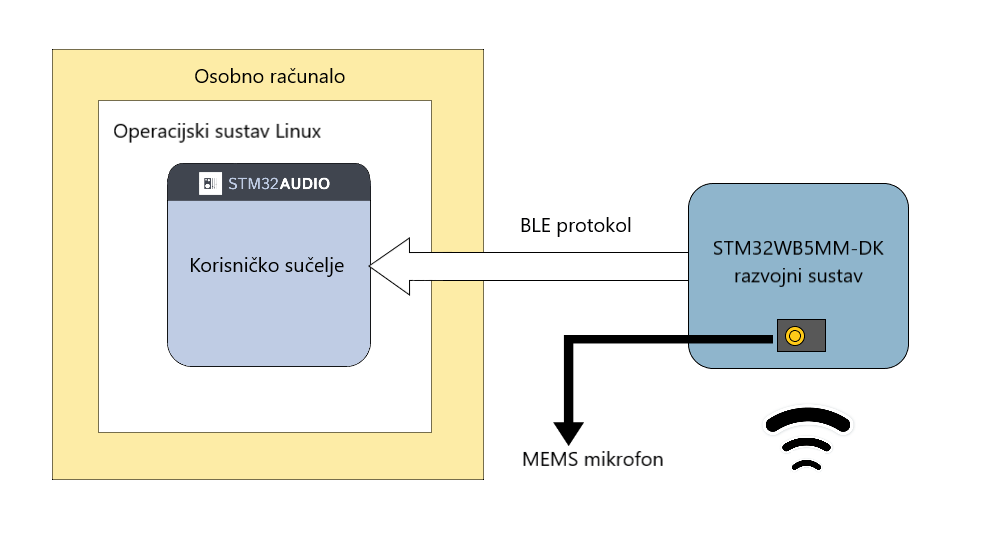
\includegraphics[width=\linewidth]{imgs/shema}
	\caption{Blok shema sustava}
	 \label{fig:shema}
\end{figure}

\cite{signalprocessing}
\eject
\chapter{Razvojni sustav STM32WB5MM-DK}

Razvojni sustav temelji se na modulu STM32WB5MMG tvrtke \textit{STMicroelectronics}, koji je dio linije STM32WBx5 razvojnih sustava. Kao i svi mikrokontroleri iz te skupine, modul sadrži 32-bitni aplikacijski procesor ARM Cortex-M4 koji radi na frekvenciji do 64 MHz te mrežni procesor Cortex-M0+ s frekvencijom rada do 32MHz. Modul sadrži 1 MB memorije tipa \textit{Flash} i 256 KB memorije tipa SRAM (engl. \textit{Static random-access memory}).\cite{stm32manual} Budući da modul ima funkciju RF (engl. \textit{radio frequency}) primopredajnika, podržava protokole Bluetooth, Zigbee, Thread i konkurentne bežične standarde. Sustav također ima 0.96-inčni 128x64 zaslon, RGB LED diode te senzore za temperaturu, dodir, \textit{Time-of-Flight} senzor i žiroskop. Od ostale periferije najznačajniji je digitalni IMP34DT05 MEMS mikrofon. Modul STM32WB5MMG je višeprotokolni, bežični uređaj niske potrošnje energije (engl. \textit{ultra-low-power}) primarno namijenjen razvoju aplikacija koje koriste audio, USB ili \textit{Bluetooth Low Energy} (BLE) protokol. Konfiguracija razvojnog sustava s istaknutim položajem MEMS mikrofona prikazana je na slici \ref{fig:discovery-kit}.

\begin{figure}[ht]
	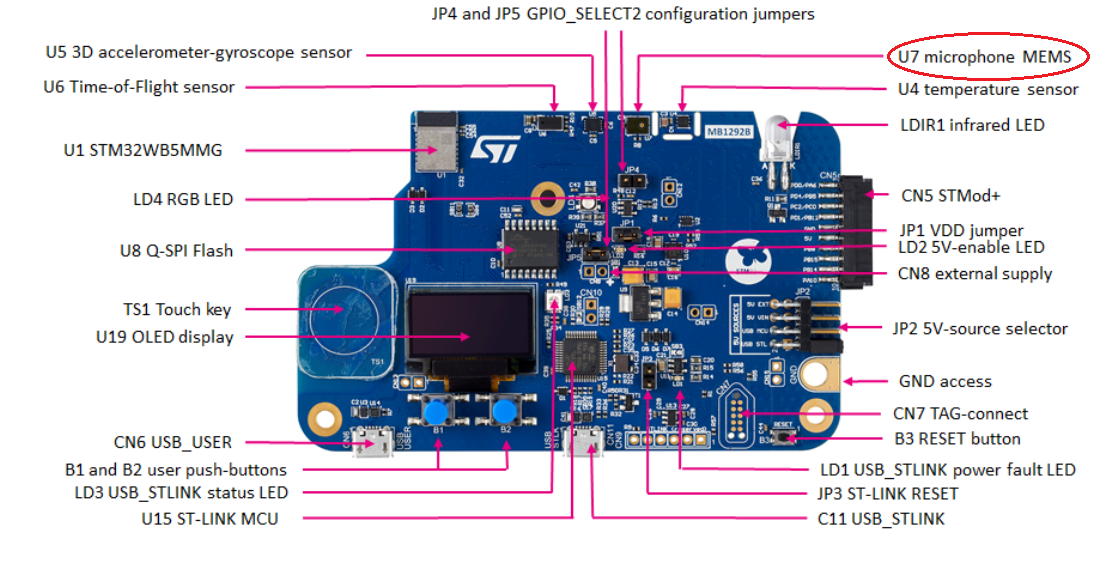
\includegraphics[scale=0.5]{imgs/discovery_kit}
	\caption{Konfiguracija razvojnog sustava STM32WB5MM-DK \cite{stm32manual}}
	\label{fig:discovery-kit}
\end{figure}

\section{BLE protokol}

Bluetooth protokol korišten je za povezivanje razvojnog sustava s razvojnim računalom i za prijenos audio signala s mikrokontrolera. BLE je vrsta bežične komunikacije namijenjena komunikaciji kratkog dometa s niskom potrošnjom energije. Razvijen je kako bi se postigao standard vrlo male snage koji radi s baterijom veličine kovanice (engl. \textit{coin-cell batteries}) nekoliko godina.
Klasična Bluetooth tehnologija razvijena je kao bežični standard, što je omogućilo razvoj bežičnih i prenosivih uređaja, no ne podržava dug život baterije zbog brze i nepredvidive komunikacije te složenih postupaka povezivanja. BLE uređaji troše samo dio energije koju troše standardni Bluetooth proizvodi te omogućavaju malenim uređajima s malim baterijama bežično povezivanje s uređajima koji koriste klasični Bluetooth \cite{blevsbluetooth}. 

BLE radi u istom opsegu od 2,4 GHz kao i standardni Bluetooth, no koristi različite kanale od standardnog Bluetootha. Koristi 40 kanala od 2 MHz za prijenos podataka korištenjem modulacije Gaussova pomaka frekvencije (metoda koja se koristi za glatkije prijelaze između podatkovnih impulsa), zbog čega skokovi frekvencije proizvode manje smetnji u usporedbi sa standardnom Bluetooth komunikacijom.

Atributi su adresirani dijelovi informacija koji mogu sadržavati korisničke podatke ili meta-informacije o arhitekturi samih atributa, te se koriste za razmjenu informacija između dva uređaja putem BLE sučelja. Uređaj koji prikazuje atribute naziva se poslužiteljem, a uređaj koji ih koristi naziva se klijentom. 

Atributi se sastoje od nekoliko parametara:
\begin{itemize}
	\item parametar \textit{handle}: jedinstveni 16-bitni identifikator za svaki atribut na određenom poslužitelju; svaki atribut čini adresabilnim i zajamčeno se neće mijenjati,
	\item tip: 16, 32 ili 128-bitni univerzalni jedinstveni identifikator (UUID) koji određuje vrstu podataka prisutnih u vrijednosti atributa,
	\item dopuštenja: meta-podaci koji opisuju dopuštenja za pristup ATT podacima, enkripciju i autorizaciju,
	\item vrijednost: stvarni sadržaj podataka atributa; dio atributa kojem klijent može pristupiti za čitanje i/ili pisanje.
\end{itemize}

Arhitektura BLE tehnologije, prikazana na slici \ref{fig:ble-stack-arch}, naziva se još i BLE stog zbog slojevite strukture. Stog se sastoji od dvije glavne komponente:
\begin{itemize}
	\item BLE upravljač (engl. \textit{controller}) koji prenosi podatke,
	\item BLE domaćin (engl. \textit{host}) koji definira odnos povezanih uređaja  \cite{blemanual}.
\end{itemize}

\begin{figure}[ht]
	\centering
	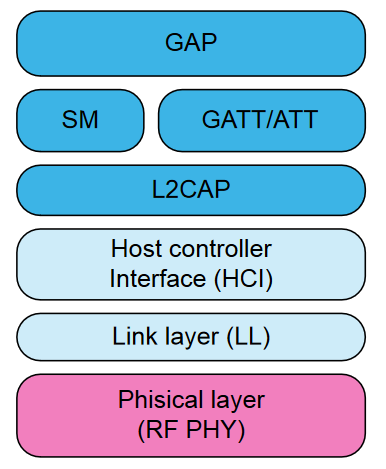
\includegraphics[scale=0.6]{imgs/ble_stack_arch}
	\caption{Arhitektura BLE stoga \cite{blemanual}}
	\label{fig:ble-stack-arch}
\end{figure}

Fizički sloj dio je upravljača i emitira signal u radiofrekvencijskom području brzine od 1 Mbps koji prenosi informacije GFSK (engl. \textit{Gaussian Frequency Shift Keying}) frekvencijskom modulacijom. Radi u 2,4 GHz ISM pojasu bez licence na 2400-2483,5 MHz. 
BLE sustav koristi 40 RF kanala (0-39), s razmakom od 2 MHz. Postoje dvije vrste kanala:
\begin{enumerate}
	\item Kanali za oglašavanje koji koriste tri fiksna RF kanala (37, 38 i 39) za sljedeće tipove paketa:
	\begin{enumerate}
		\item Pakete kanala za oglašavanje
		\item Pakete korištene za otkrivanje ili povezivanje
		\item Pakete korištene za odašiljanje ili skeniranje
	\end{enumerate}
	\item Podatkovni fizički kanal, koristi ostalih 37 RF kanala za dvosmjernu komunikaciju između povezanih uređaja.
\end{enumerate}

BLE je tehnologija adaptivnog skakanja frekvencije (engl. \textit{Adaptive frequency-hopping} - AFH) koja može koristiti samo podskup svih dostupnih frekvencija kako bi se izbjegle sve frekvencije koje koriste druge neprilagodljive tehnologije. To omogućuje prelazak s lošeg kanala na poznati dobar kanal korištenjem specifičnog algoritma za skakanje frekvencije, koji određuje sljedeći dobar kanal za korištenje.

Sloj veze, također dio upravljača, određuje kako dva uređaja mogu koristiti signale u radiofrekvencijskom području za međusoban prijenos informacija. Također definira automat s pet stanja:
\begin{itemize}
	\item stanje pripravnosti (engl. \textit{standby}): uređaj ne šalje niti prima pakete,
	\item oglašavanje (engl. \textit{advertisement}): uređaj šalje oglase putem kanala za oglašavanje,
	\item skeniranje (engl. \textit{scaanning}): uređaj traži uređaje oglašivača,
	\item pokretanje (engl. \textit{initiating}): uređaj pokreće vezu s uređajem oglašivača,
	\item veza (engl. \textit{connection}): 
	\begin{itemize}
		\item uređaj  koji je inicirao komunikaciju je u ulozi \textit{master}, komunicira sa  \textit{slave} uređajem i definira vrijeme prijenosa,
		\item uređaj oglašivača je u ulozi \textit{slave}, komunicira s jednim \textit{master} uređajem.
	\end{itemize}

\end{itemize}

\begin{figure}[ht]
	\centering
	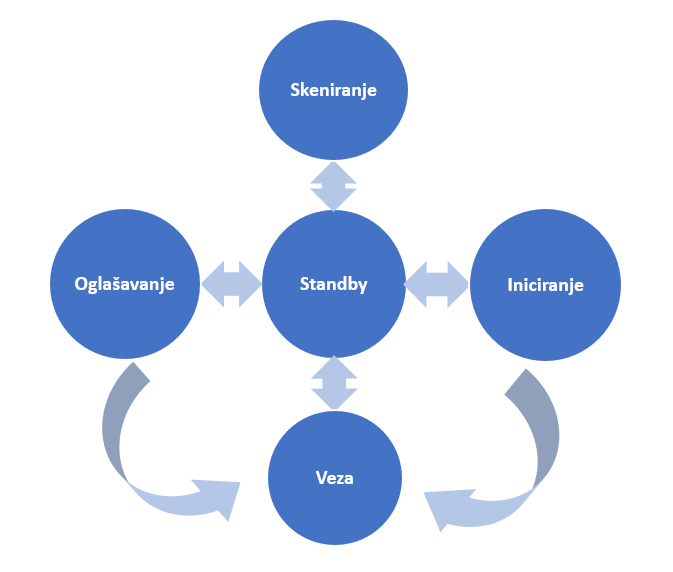
\includegraphics[scale=0.7]{imgs/ll_state_machine}
	\caption{Automat sloja veze \cite{blemanual}}
	\label{fig:ll-state-machine}
\end{figure}

Sučelje između domaćina i upravljača (HCI) je neovisan međusloj koji povezuje te BLE komponente i pruža sredstvo komunikacije putem softverskog aplikacijskog programskog sučelja (engl. \textit{Application Programming Interface} - API) ili hardverskog sučelja kao što su: SPI, UART ili USB. Dolazi iz standardnih Bluetooth specifikacija, s novim dodatnim naredbama za funkcije koje osiguravaju nisku potrošnju energije.

Protokol logičke veze i sloja prilagodbe (L2CAP) dio je BLE domaćina koji podržava multipleksiranje protokola više razine, operacije fragmentacije paketa i ponovnog sastavljanja, te prijenos informacija o kvaliteti usluga.

BLE sloj veze (SM) podržava enkripciju i autentifikaciju korištenjem načina brojača s CBC-MAC algoritmom (kod za provjeru autentičnosti lančanih poruka) i 128-bitnu AES blok šifru (AES-CCM). Kada se enkripcija i autentifikacija koriste u vezi, 4-bajtna provjera integriteta poruke (MIC) dodaje se na jedinici podatkovnog protokola (PDU). Enkripcija se primjenjuje i na polja od PDU i MIC. Kada dva uređaja žele šifrirati podatke tijekom veze, upravitelj sigurnosti (SM) koristi postupak uparivanja. Ovaj postupak omogućuje provjeru autentičnosti dvaju uređaja razmjenom informacija o njihovu identitetu kako bi se stvorili sigurnosni ključevi koji se mogu koristiti kao osnova za pouzdani odnos ili jednu sigurnu vezu. 

Protokol atributa (ATT) definira skup metoda za otkrivanje, čitanje i pisanje atributa na drugi uređaj. Implementira \textit{peer-to-peer} protokol između poslužitelja i klijenta tipičnom zahtjev-odgovor strukturom. 

Generički atributni profil (GATT) definira okvir za korištenje ATT protokola, a koristi se za usluge, otkrivanje deskriptora, čitanje, pisanje i obavijesti. Podaci poslani putem BLE-a organizirani su ovim slojem.
U GATT kontekstu, kada su dva uređaja povezana, postoje dvije uloge uređaja:
\begin{itemize}
	\item GATT klijent: uređaj pristupa podacima na udaljenom GATT poslužitelju putem čitanja, pisanja, obavještavanja,
	\item  GATT poslužitelj: uređaj pohranjuje podatke lokalno i pruža metode pristupa podacima udaljenom GATT klijentu.
\end{itemize}

Atributi GATT poslužitelja organizirani su kao niz usluga, od kojih svaka počinje atributom deklaracije usluge koji označava njen početak. Svaka usluga grupira jednu ili više karakteristika i svaka karakteristika može uključivati nula ili više deskriptora.

Bluetooth sustav definira osnovni profil koji implementiraju svi Bluetooth uređaji. Ovaj profil naziva se generički profil pristupa (GAP), koji definira osnovne zahtjeve Bluetooth uređaja. Programska potpora mikrokontrolera implementira komunikacijsku paradigmu temeljenu na povezivanju koja pruža trajnu vezu od točke do točke (engl. \textit{point-to-point}) između dva uređaja kojom upravlja GAP sloj. Postoje četiri uloge GAP profila:
\begin{itemize}
	\item emiter (engl. \textit{broadcaster}): šalje oglase,
	\item promatrač (engl. \textit{observer}): prima oglase,
	\item periferija (engl. \textit{peripheral}): uvijek u načinu oglašavanja i u ulozi \textit{slave}, 
	\item centar (engl. \textit{central}): nikada ne šalje oglase, uvijek u \textit ulozi {master}.
\end{itemize}

Razvijena programska potpora koristi dvije od navedenih uloga, a to su periferija i centar. Periferna uloga postavljena je mikrokontroleru jer se ta uloga postavlja uređajima koji podržavaju jednu vezu i smanjenu složenost. Ovi uređaji zahtijevaju samo upravljač koji podržava ulogu \textit{slave} i koristi središnju frekvenciju upravljača za razmjenu podataka. S druge strane, centralna uloga pridružuje se uređaju koja podržava višestruke veze i pokretanje veza s perifernim uređajima. Ovi uređaji zahtijevaju upravljač koji podržava glavnu ulogu sa složenijim funkcijama, što je u ovom slučaju računalo.

Na slici \ref{fig:ble_connection_setup} prikazana je komunikacija između dva uređaja, odnosno računala i mikrokontrolera. Prema BLE specifikaciji, periferija ulazi u način oglašavanja (engl. \textit{advertisment mode}) pri pokretanju i šalje pakete oglasa u relativno dugim intervalima. Središnja jedinica ulazi u način otkrivanja (engl. \textit{discovery mode}) i šalje zahtjev za povezivanjem nakon primitka paketa oglasa od \textit{slave} uređaja. Nakon što je veza uspostavljena, obavijesti koje nose audio podatke periodično se šalju od poslužitelja do klijenta u odabranom smjeru: periferija-centar, centar-periferija ili istovremeno na oba načina. Dok je mikrokontroler u načinu oglašavanja sve do uspostave veze, računalo je u načinu otkrivanja samo kraći vremenski period te prekida sa skeniranjem dostupnih uređaja nakon zadanog vremenskog intervala. Mikrokontroler ima ulogu \textit{slave}, dok računalo ima ulogu \textit{master}. 

\begin{figure}[ht]
	\centering
	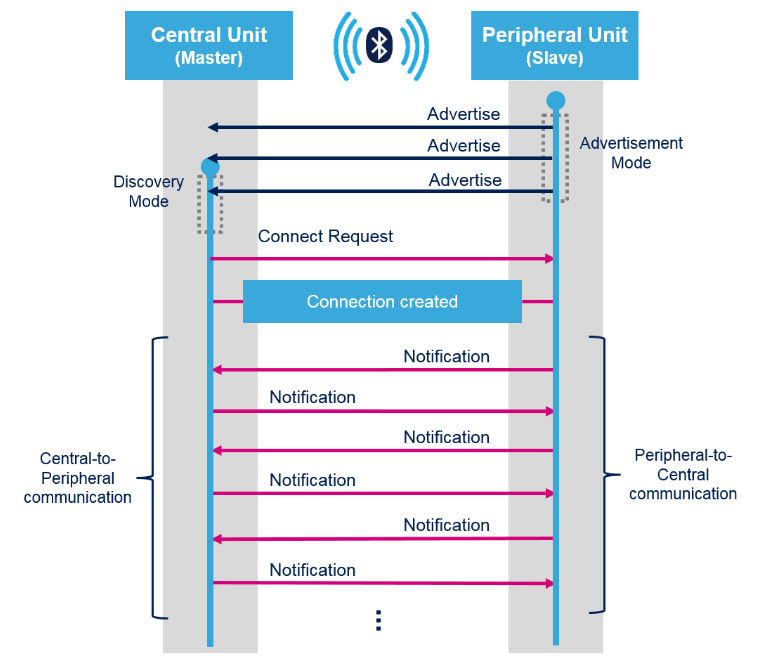
\includegraphics[scale=0.7]{imgs/ble_connection_setup}
	\caption{Uspostava BLE veze \cite{fpaudbvlink}}
	\label{fig:ble_connection_setup}
\end{figure}


\section{MEMS mikrofon}

MEMS (engl. \textit{Micro-Electro-Mechanical Systems}) mikrofon je elektroakustični pretvornik koji sadrži MEMS senzor i aplikacijski specifičan integrirani sklop (ASIC). MEMS mikrofoni se uglavnom temelje na elektretskim kapsulama i obično imaju ugrađena pretpojačala i analogno-digitalne pretvornike. MEMS mikrofoni su također poznati kao mikrofonski čipovi ili silikonski mikrofoni \cite{whatismems}. 

Na razvojnom sustavu ugrađen je IMP34DT05 mikrofon. To je digitalni MEMS mikrofon niske potrošnje energije koji prima audio signal iz svih smjerova (engl.~\textit{omnidirectional}). Izgrađen je s kapacitivnim senzorskim elementom i sučeljem integriranog kruga koje povezuje mikrofon s razvojnim sustavom. IMP34DT05 je digitalni mikrofon niske distorzije s omjerom signala i šuma od 64 dB i osjetljivošću od –26 dBFS ±3 dB, što označava relativno visoku osjetljivost \cite{memsdb}.

Svi mikrofoni detektiraju akustične valove pomoću fleksibilne membrane, odnosno dijafragme. Membrana se pomiče pod pritiskom induciranih akustičnih valova. Danas većina MEMS mikrofona na tržištu koristi kapacitivnu tehnologiju za prikupljanje zvučnih signala. Kapacitivni MEMS mikrofoni mjere kapacitet između fleksibilne mikromembrane i fiksne stražnje ploče. Promjene tlaka zraka koje stvaraju zvučni valovi uzrokuju pomicanje membrane. Stražnja ploča je perforirana kako bi kroz nju mogao strujati zrak i dizajnirana je da ostane kruta budući da zrak prolazi kroz njezine perforacije. Kako se membrana pomiče, kapacitet se mijenja između pokretne membrane i fiksne stražnje ploče (budući da se udaljenost između njih mijenja), a ta se promjena može analizirati i zabilježiti.

Dizajn digitalnog MEMS mikrofona obično ima dodatni CMOS čip kao analogno-digitalni pretvornik. Ovi čipovi učinkovito preuzimaju pojačane analogne audio signale i pretvaraju ih u digitalne podatke. Također omogućuju lakšu integraciju digitalnih MEMS mikrofona s digitalnim proizvodima.

Najčešći format za digitalno kodiranje unutar MEMS mikrofona je modulacija trajanja impulsa (engl. \textit{pulse-duration modulation} - PDM). PDM omogućuje komunikaciju jednom podatkovnom linijom i satom. Prijamnici PDM signala, kao i sami MEMS mikrofoni, jeftini su i lako dostupni.

\subsection{MEMS tehnologija}
Mikroelektromehanički sustavi ili MEMS je tehnologija koja se definira kao sustav minijaturiziranih mehaničkih i elektromehaničkih elemenata (tj. uređaja i struktura) koji su izrađeni mikrotvorničkim tehnikama. Fizičke dimenzije MEMS uređaja mogu varirati od znatno ispod jednog mikrometra pa sve do nekoliko milimetara. Isto tako, tipovi MEMS uređaja mogu varirati od relativno jednostavnih struktura bez pokretnih elemenata, do iznimno složenih elektromehaničkih sustava s više pokretnih elemenata pod kontrolom integrirane mikroelektronike. Jedan glavni kriterij MEMS-a je da postoje barem neki elementi koji imaju neku vrstu mehaničke funkcionalnosti bez obzira na to mogu li se ti elementi kretati ili ne.

Dok su funkcionalni elementi MEMS-a minijaturizirane strukture, senzori, aktuatori i mikroelektronika, najznačajniji elementi su mikrosenzori i mikroaktuatori. Oni su  kategorizirani kao pretvornici energije iz jednog oblika u drugi - primjerice mikrosenzor, koji obično pretvara izmjereni mehanički signal u električni.

Stvarni potencijal MEMS-a ostvaruje se kada se minijaturizirani senzori, aktuatori i strukture spoje na silicijsku podlogu zajedno s integriranim krugovima, odnosno mikroelektronikom. Mikromehaničke komponente proizvode se korištenjem kompatibilnih \textit{micromachining} procesa koji selektivno urezuju dijelove silikonske pločice ili dodaju nove strukturne slojeve kako bi formirali mehaničke i elektromehaničke uređaje. Još je kompleksnije ako se MEMS može spojiti ne samo s mikroelektronikom, već i s drugim tehnologijama kao što su fotonika, nanotehnologija itd. Ovakve konfiguracije ponekad se nazivaju heterogenom integracijom. Dok su složenije razine integracije budući trend MEMS tehnologije, sadašnja je tehnologija skromnija i obično uključuje jedan diskretni mikrosenzor, jedan diskretni mikroaktuator, jedan mikrosenzor integriran s elektronikom, mnoštvo identičnih mikrosenzora integriranih s elektronikom, jedan mikroaktuator integriran s elektronikom ili mnoštvo identičnih mikroaktuatora integriranih s elektronikom \cite{whatismems_tech}. 
 

\subsection{Načela rada MEMS mikrofona}

MEMS mikrofon sadrži sljedeće komponente:
\begin{itemize}
	\item MEMS pretvornik: sastoji se od membrane, perforirane ploče i kućišta,
	\item tiskana pločica (engl. \textit{printed circuit board} - PCB): uključuje ASIC polarizacijsku jedinicu, mikrofonsko pretpojačalo i A/D pretvornik,
	\item mehanički poklopac.
\end{itemize}

Zvučni valovi ulaze u MEMS mikrofon kroz poklopac i prolaze kroz perforirano kućište i ploču prije nego dođu do membrane. Valovi uzrokuju razliku u tlaku između prednje i stražnje strane membrane. Ova razlika tlaka uzrokuje njeno pomicanje sukladno zvučnim valovima. Međutim, mikrofonski signal se stvara samo ako postoji naboj između vodljive membrane i stražnje ploče. 
Ploča i membrana zajedno djeluju kao kondenzator koji je potrebno napuniti za ispravan
rad. Pripadajući integrirani sklop (ASIC) osigurava ovo punjenje.

Jednom napunjene, ploča i membrana mogu proizvesti napon. Budući da djeluju kao kondenzator, svaka promjena kapaciteta prouzročit će obrnuto proporcionalnu promjenu napona. Kapacitet je funkcija udaljenosti između ploče i membrane, stoga dok membrana oscilira, stvara se izmjenični napon odnosno mikrofonski signal. Ovaj napon treba pojačati da bi bio koristan kao audio signal, stoga odvojeni integrirani krug (poluvodička matrica), uključen u PCB, pojačava signal.

Ako se koristi analogni MEMS mikrofon, pojačani audio signal bi se u ovom obliku doveo na izlaz MEMS mikrofona.  Međutim, u digitalnom MEMS mikrofonu postoji dodatni proces u kojem ADC pretvara analogni signal PDM metodom prije nego što emitira digitalni audio signal.

Kao što se vidi na slici \ref{fig:mems-mic}, stacionarna ploča je perforirana, što omogućava zraku prolaz do membrane. Na ovom je prikazu ASIC čip pričvršćen na ploču, no to nije slučaj kod svakog MEMS mikrofona. 

Stražnja je komora u ovom primjeru zatvorena, što znači da je MEMS mikrofon tlačni mikrofon - membrana je otvorena samo za zvučne valove s jedne strane, što znači da prima zvuk iz svih smjerova. Stražnja komora također djeluje kao akustični rezonator i tako pomaže pri pravilnom podešavanju mikrofona.

Također je potreban i otvor za ventilaciju kako bi stražnja komora bila pod tlakom okoline \cite{memsdepth}.

\begin{figure}[ht]
	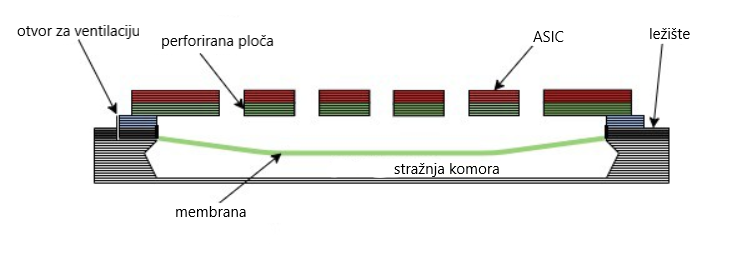
\includegraphics[width=\linewidth]{imgs/mems_mic}
	\caption{Poprečni presjek MEMS mikrofona \cite{memsdepth}}
	\label{fig:mems-mic}
\end{figure}
\chapter{Povezivanje razvojnog sustava i računala}

Računalo i STM32 razvojni sustav dva su odvojena sustava koja moraju međusobno komunicirati i razmjenjivati podatke. Za ostvarenje njihove veze razvijena su dva programska rješenja:
\begin{enumerate}
	\item programska potpora za mikrokontroler, koja će omogućiti pokretanje i snimanje zvučnog zapisa te njegov prijenos BLE sučeljem,
	\item programska potpora za računalo, koja će ostvariti Bluetooth vezu između računala i mikrokontrolera te omogućiti prijem i pohranu primljenog audio signala.
\end{enumerate} 

\section{Programska potpora za mikrokontroler}

Dvije glavne funkcionalnosti koje mikrokontroler mora sadržavati su snimanje zvuka i njegov prijenos BLE komunikacijskim sučeljem. Za rad mikrokontrolera odabran je paket funkcija \textit{FP-AUD-BVLINKWB1} iz alata \textit{STM32Cube} koji je razvila tvrtka \textit{STMicroeletronics}. Ovaj \textit{firmware} omogućava potpuni dvosmjerni prijenos zvuka koji se prenosi BLE sučeljem koristeći Opus algoritam za kompresiju. Aplikacija sadrži \textit{drivere} i posrednički softver (engl. \textit{middleware}) za BLE i digitalne MEMS mikrofone. Također uključuje kompletan Opus audio kodek kao \textit{middleware} za izvođenje dvosmjernog i simultanog prijenosa zvuka između dva STM32WB mikrokontrolera. 

\subsection{Arhitektura programske potpore za mikrokontroler}

Softver se temelji na sloju apstrakcije hardvera STM32CubeHAL za STM32 mikrokontroler. Paket funkcija opremljen je skupom \textit{middleware} komponenti za audio prijem, kompresiju i
dekompresiju, prijenos podataka preko BLE sučelja i USB-a.

Aplikacija se sastoji od sljedećih slojeva softvera:
\begin{itemize}
	\item STM32Cube HAL sloj: pruža jednostavan i generički skup generičkih i proširenih API-ja (sučelja za programiranje aplikacije) za interakciju s gornjim slojevima aplikacije i bibliotekama. Ovi su API-ji izgrađeni na zajedničkoj arhitekturi te je moguće na njih dodavati slojeve (primjerice specifični \textit{middleware}) bez potrebe za specifičnim hardverskim informacijama mikrokontrolera.
	\item Sloj paketa podrške za ploču (BSP): skup API-ja koji pruža programsko sučelje za periferne uređaje specifične za ploču kao što su SPI, ADC, LED i korisnički gumbi.
\end{itemize}

\begin{figure}[ht]
	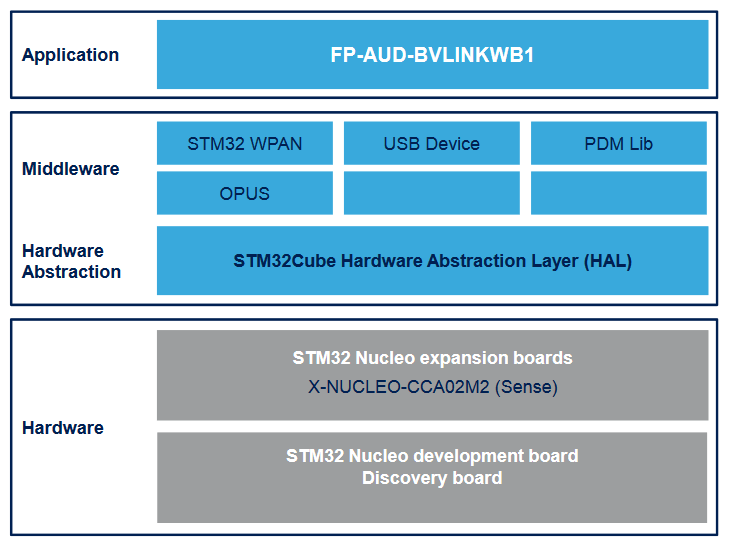
\includegraphics[width=\linewidth]{imgs/firmware_software_arch}
	\caption{Arhitektura softvera FP-AUD-BVLINKWB1}
	\label{fig:firmware_software_arch}
\end{figure}

Komponente za obradu funkcijskog paketa \textit{FP-AUD-BVLINKWB1} dizajnirane su za stvaranje bežične audio veze između modula odašiljača (Tx) i prijemnika (Rx), gdje mikrokontroler služi kao odašiljač, a računalo kao prijemnik. Cijeli lanac obrade zvuka počinje prijemom MEMS digitalnim mikrofonom i kulminira reprodukcijom zvuka na računalu.

BLE je konfiguriran za slanje paketa s maksimalnom veličinom od 150 bajtova. Ovisno o aplikaciji, kodirani bajtovi mogu biti iznad ovog praga, stoga komprimirani međuspremnik (engl. \textit{buffer}) mora biti podijeljen u više BLE paketa. Štoviše, veličina kodiranog međuspremnika može promijeniti svaki audio okvir i prijemnik mora znati njegovu duljinu da bi ga obnovio; za ovaj opseg implementiran je jednostavan protokol BLE prijenosa.

Na strani odašiljača, zvuk se dobiva digitalnim MEMS mikrofonom kao 1-bitni PDM signal i pretvara se pomoću filtra za pretvorbu PDM-u-PCM u 16-bitni PCM. Svaki put kad je audio okvir spreman, prenosi se u algoritam kompresije: veličina kodiranog međuspremnika koju vraća Opus koder može se značajno promijeniti u skladu s parametrima Opus kodera.

\begin{figure}[ht]
	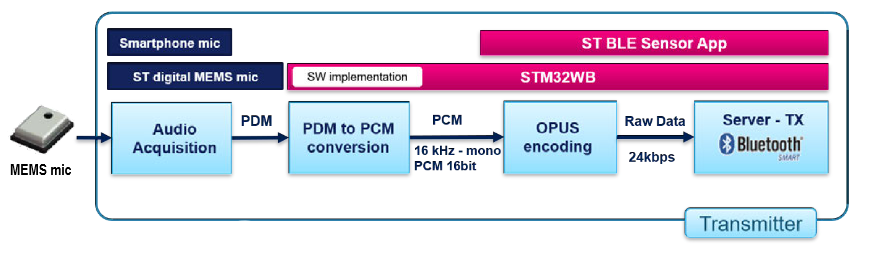
\includegraphics[width=\linewidth]{imgs/duplex_chain}
	\caption{Lanac obrade odašiljača u \textit{FP-AUD-BVLINKWB}}
	\label{fig:duplex_chain}
\end{figure}

\subsection{\textit{Middleware} za prijenos zvuka}

Budući da \textit{streaming} zvuka nije dio predefiniranog skupa profila mikrokontrolera, \textit{FP-AUD-BVLINKWB1} definira uslugu specifičnu za dobavljača pod nazivom \textit{BlueVoiceOPUS} koja je posrednik između korisničkog zvuka i  klijentskog uređaja. Ovisno o pokrenutoj aplikaciji, karakteristika se mijenja između audio ili glazbene karakteristike. Budući da \textit{streaming} glazbe nije implementiran u ovoj aplikaciji, opisane su samo audio karakteristike. 

Audio karakteristike sadrže sljedeće atribute:
\begin{itemize}
	\item \textit{Att1} sadrži deklaraciju audio karakteristika
	\begin{itemize}
		\item UUID: standardni 16-bitni UUID za karakterističnu deklaraciju
		\item Dozvole: R
		\item Vrijednost: svojstva za ovu karakteristiku su "\textit{notify only}", a UUID je za audio podatke
	\end{itemize}
	\item \textit{Att2} sadrži audio podatke
	\begin{itemize}
		\item UUID: isti UUID u zadnjih 16 bajtova vrijednosti atributa definicije karakteristike
		\item Dozvole: nema
		\item Vrijednost: stvarni audio sadržaj
	\end{itemize}
	\item \textit{Att3} sadrži konfiguraciju karakteristika klijenta
	\begin{itemize}
		\item UUID: standardni 16-bitni UUID za karakterističnu konfiguraciju klijenta
		\item Dozvole: R/W
		\item Vrijednost: prvi bit označava omogućenost obavijesti (0 ili 1), drugi bit omogućenost indikacija
	\end{itemize}
\end{itemize}

Usluga \textit{BlueVoiceOPUS} može implementirati odašiljač, prijamnik ili oboje u slučaju \textit{full-duplex} komunikacije. Za ovu aplikaciju potrebno je implementirati odašiljač odnosno transmiter.
Za prijenos zvuka, usluga i karakteristike moraju se kreirati pozivanjem \lstinline|BVOPUS_STM_Init|, što uključuje funkcije \lstinline|BluevoiceOPUS_AddService| i \lstinline|BluevoiceOPUS_AddChar|; UUID-ovi su definirani u datoteci \lstinline|bvopus_service_stm.c|.

Karakteristike se mogu dodati već postojećoj usluzi pozivanjem \lstinline|BluevoiceOPUS_AddChar| i prosljeđivanjem oznake te određene usluge kao parametra. Ako funkcija vrati \lstinline|BV_OPUS_SUCCESS|, BLE profil je ispravno kreiran.

Također, potrebno je konfigurirati Opus koder. U skladu sa traženim funkcijama, koder se može kreirati ispunjavanjem relevantne strukture \lstinline|OPUS_IF_ENC_ConfigTypeDef|.

Koder se može inicijalizirati pozivom \lstinline|BVOPUS_CodecEncInit(&EncConfigOpus)|. Ako funkcija vrati \lstinline|BV_OPUS_SUCCESS|, \textit{BlueVoiceOPUS} profil ispravno je konfiguriran. Ako vrati \lstinline|BV_OPUS_INVALID_PARAM|, neki od parametara nisu ispravni. Ovisno o odabranim parametrima, inicijalizacijska funkcija dodjeljuje količinu memorije koju relevantni API vraća interno. 

Pri inicijalizaciji podržani su sljedeći parametri:
\begin{itemize}
	\item \textit{application}: \lstinline|OPUS_APPLICATION_VOIP, OPUS_APPLICATION_AUDIO, OPUS_APPLICATION_RESTRICTED_LOWDELAY|
	\item \textit{bitrate} [bps]: od 6000 do 510000
	\item \textit{channels}: od 1 do 255
	\item \textit{complexity}: od 0 do 10
	\item \textit{ms\_frame} [ms]: 2.5, 5, 10, 20, 40, 60
	\item \textit{sample\_freq} [Hz]: 8000, 12000, 16000, 24000, 48000
\end{itemize}

\begin{lstlisting}[caption={Parametri za Opus koder}, language=c]
	EncConfigOpus.application = OPUS_APPLICATION_VOIP;
	/* bps */
	EncConfigOpus.bitrate = 24000; 
	/* 1 channel, mono*/
	EncConfigOpus.channels = AUDIO_CHANNELS_IN; 
	EncConfigOpus.complexity = 0;
	/* 20 ms */
	EncConfigOpus.ms_frame = AUDIO_IN_MS; 
	/* 16000 Hz */
	EncConfigOpus.sample_freq = AUDIO_IN_SAMPLING_FREQUENCY; 
\end{lstlisting}

Nakon postavljanja veze, modul koji je otkrio \textit{BlueVoiceOPUS} profil drugog modula mora omogućiti kontrolnu obavijest pozivanjem API-ja \lstinline|BluevoiceOPUS_EnableCtrl_Notif(void)|. Kontrolna se obavijest zatim koristi za zahtjev za pokretanje i zaustavljanje prijenosa.

Za početak audio prijenosa, modul odašiljača mora zatražiti od prijamnika da omogući njegovu audio obavijest pozivom \lstinline|BluevoiceOPUS_SendEnableNotifReq|. Ovaj API šalje obavijest putem kontrolne karakteristike koja sadrži dva bajta (\lstinline|{BV_OPUS_CONTROL, BV_OPUS_ENABLE_NOTIF_REQ}|). Čim čvor primi zahtjev može omogućiti audio obavijest podnositelju zahtjeva pozivom funkcije \lstinline|BluevoiceOPUS_EnableAudio_Notif(void)|. Ako je obavijest ispravno omogućena, modul može započeti prijenos zvuka.

\textit{BlueVoiceOPUS} profil na ulaz prihvaća količinu PCM uzoraka jednaku veličini audio okvira postavljenoj tijekom Opus konfiguracije. Svaki put kada je audio okvir spreman, treba pozvati API \lstinline|BluevoiceOPUS_SendAudioData| i on automatski sažima, fragmentira i šalje pakete audio podataka.

Za svaku primljenu zvučnu obavijest potrebno je pozvati \lstinline|BluevoiceOPUS_ParseData| i provjeriti vraćeni status. U slučaju uspjeha, parametar \lstinline|pcm_samples| pokazuje je li spreman kompletan audio okvir.

Prema zadanim postavkama, Opus koder je konfiguriran s promjenjivom brzinom prijenosa: svaki kodirani okvir ima  duljinu prilagođenu brzini prijenosa postavljenoj tijekom faze inicijalizacije. Maksimalna veličina BLE paketa postavljena je na 150 bajtova, a broj BLE paketa može varirati među različitim audio okvirima ili ovisno o konfiguraciji Opusa.

Protokol prijenosa \textit{BlueVoiceOPUS} modula pokazuje kada kodirani podaci počinju i završavaju tako da prijamnik može ponovno izgraditi komprimirani međuspremnik i dekodirati ga: jedan bajt se dodaje kao prvi bajt svakog BLE paketa, preostalih 19 bajtova ili više, ovisno o odabranom MTU, popunjeni su podacima kodiranim Opusom.

Sljedeće vrijednosti mogu biti bajt zaglavlja:
\begin{itemize}
	\item \lstinline|BV_OPUS_TP_START_PACKET = 0x00|
	\item \lstinline|BV_OPUS_TP_START_END_PACKET = 0x20|
	\item \lstinline|BV_OPUS_TP_MIDDLE_PACKET = 0x40|
	\item \lstinline|BV_OPUS_TP_END_PACKET = 0x80|
\end{itemize}

Protokol prijenosa u potpunosti je obrađen u \textit{BlueVoiceOPUS} usluzi.
\subsection{Opus}
Opus je otvoren i svestran audio kodek koji se može koristiti za različite vrste aplikacija kao što su \textit{streaming} govora i glazbe ili komprimirana pohrana zvuka. Skalabilnost, od uskopojasnog govora niske brzine prijenosa pri 6 kbit/s do stereo glazbe pri 510 kbit/s niske složenosti, čini ga pogodnim za širok raspon interaktivnih aplikacija.

Sastoji se od dva sloja: jedan se temelji na linearnom predviđanju (LP), a drugi se temelji na modificiranoj diskretnoj kosinusnoj transformaciji (MDCT). Opus kombinira rezultate s gubitcima i bez gubitaka. Primjerice, u govornim aplikacijama, LP tehnike poput CELP-a (engl. \textit{Code-excited linear prediction}) učinkovitije kodiraju niske frekvencije nego u tehnikama transformacijske domene kao što je MDCT.

Opus kodek se sastoji od SILK i CELT tehnologija kodiranja. Prvi koristi model temeljen na predviđanju (LPC), dok je drugi u potpunosti modeliran na MDCT transformaciji. Ova svestranost omogućuje Opusu rad u tri načina rada (SILK, CELT ili hibridni način) i osigurava višestruke konfiguracije za različite aplikacije.

\section{Programska potpora za računalo}

Glavna zadaća aplikacije na računalu je primiti audio signal Bluetoothom, prikladno ga obraditi te moći izravno reproducirati i pohraniti. Za računalnu programsku potporu odabrana je \textit{BlueST-SDK} biblioteka koji omogućuje jednostavan pristup podacima koje izvozi BLE uređaj s implementiranim BlueST protokolom. Protokol BlueST lako je proširiv za podršku korisnički definiranih podataka. On već definira različite podatke koji dolaze iz različitih senzora kao što su inercijski senzori, senzori okoliša, informacije o bateriji, te DC i motori. Također implementira serijsku konzolu preko Bluetootha koja omogućuje funkcionalnost \textit{stdint}/\textit{stdout}/\textit{stderr} i definira konfiguracijski servis za kontrolu postavki povezanih ploča. 

Korištenjem zajedničkog modela programiranja za podržane platforme, \textit{BlueST-SDK} olakšava razvoj aplikacija na Android, iOS i Linux (s instaliranim Python) sustavima i uključuje primjere aplikacija koji demonstriraju korištenje SDK. Python izdanje \textit{BlueST-SDK} biblioteke koristi \textit{bluepy} Python biblioteku dostupnu na Linuxu za povezivanje s BLE uređajima.

Za razvoj je odabran programski jezik Python na operacijskom sustavu Linux. 

\begin{figure}[ht]
	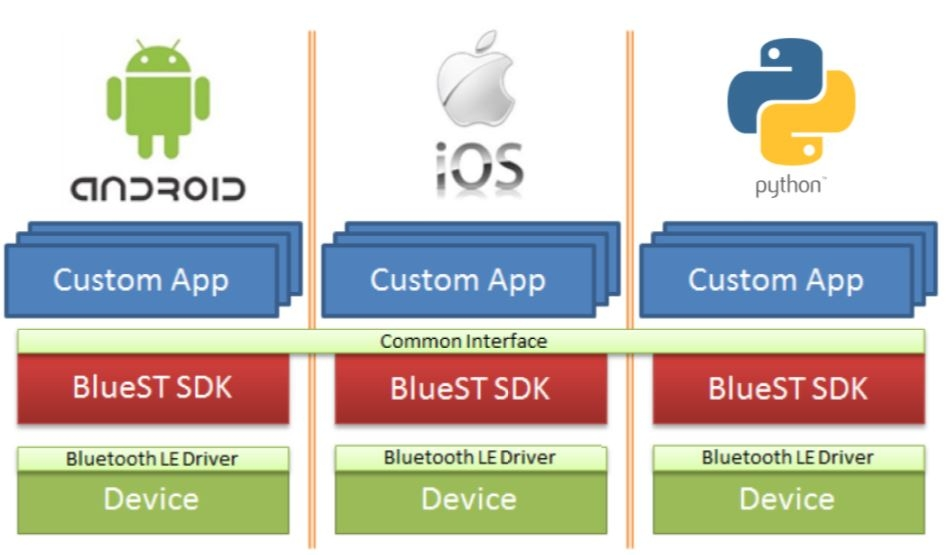
\includegraphics[width=\linewidth]{imgs/bluest_stack}
	\caption{Arhitektura aplikacije s \textit{BlueST-SDK} modulom}
	\label{fig:bluest_stack}
\end{figure}
\begin{figure}[ht]
	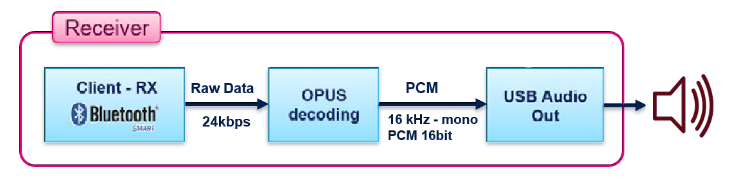
\includegraphics[width=\linewidth]{imgs/duplex_chain_2}
	\caption{Lanac obrade prijemnika u aplikaciji}
	\label{fig:duplex_chain_2}
\end{figure}
\chapter{Programska potpora za korisničko sučelje}

Za bolje korisničko iskustvo kreirano je grafičko korisničko sučelje (engl. \textit{Graphic User Interface} - GUI) koje se izvodi na korisničkom računalu. U GUI aplikaciji moguće je pokrenuti snimanje novog audiozapisa te grafički prikazati obradu signala postojećeg zvuka na računalu. 

\section{Razvojni alat PyQt} 
Aplikacija je izrađena korištenjem razvojnog alata PyQt temeljenog na programskom
jeziku Python i pripadnih biblioteka za razvoj grafičkih korisničkih sučelja. PyQt je priključak (engl. \textit{plug-in}) za Python - mostna biblioteka između Pythona i razvojnog alata Qt, koji podržava programski jezik C++. Korištena je inačica \textit{PyQt5}, koja je kompatibilna s Python 3 verzijom. \cite{pyqt} 

Osnova \textit{Qt} aplikacija je objektni model koji, koristeći sustav \textit{Meta Object} i klasu \textit{QObject}, proširuje funkcionalnost standardnog programskog jezika C++ i time omogućuje razvoj grafičkih korisničkih sučelja. \textit{PyQt} enkapsulira funkcionalnosti \textit{Qt} radnog okvira te ih prilagođava programskom jeziku Python, odnosno kombinira kompleksnost alata za razvoj grafičkog sučelja i jednostavnost programskog jezika. \cite{qt}

Osnovna klasa je \textit{QObject} koja pruža sljedeće funkcionalnosti:
\begin{itemize}
	\item definiranje objekata jedinstvenim imenom,
	\item hijerarhijska organizacija objekata,
	\item komunikacija između objekata, 
	\item upravljanje događajima.
\end{itemize}

Komunikacija između \textit{Qt} objekata odvija se mehanizmom signala i priključaka (engl. \textit{signals and slots}). Signal se emitira pri promjeni stanja objekta, primjerice pritiskom na gumb unutar korisničkog sučelja. Pri emisiji signala poziva se funkcija priključka s kojom je taj signal povezan te se obrađuje događaj koji je izazvao emisiju. 

Stvaranje i uređivanje grafičkih elemenata (engl. \textit{widgets}) omogućeno je klasom \textit{QWidget}. Grafički elementi organizirani su hijerarhijski, pri čemu je glavni prozor  „roditelj“ ostalih elemenata. 

\section{Implementacija korisničkog sučelja}

Pri pokretanju aplikacije, u glavnom prozoru prikazuje se izbornik s gumbima \textit{Record} i \textit{Analyse Audio}. \textit{Record} gumb vodi na sučelje za podešavanje parametara snimanja, dok \textit{Analyse Audio} otvara izbornik za odabir audio datoteke nad kojom će se provesti obrada signala.

\begin{figure}[ht]
	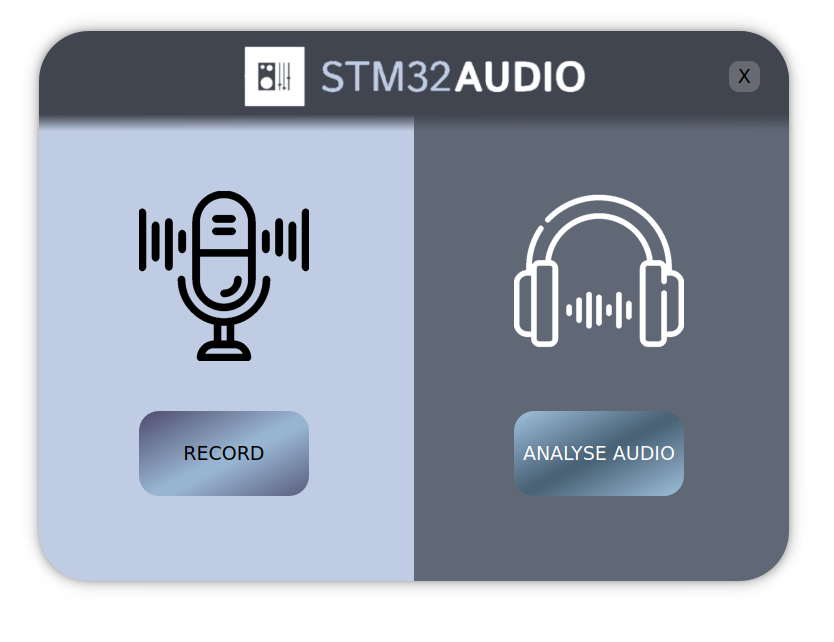
\includegraphics[width=\linewidth]{imgs/intro_form}
	\caption{Uvodni izbornik}
	\label{fig:intro_form}
\end{figure}


U sučelju za postavljanje parametara snimanja korisnik postavlja trajanje snimanja zvuka koje je ograničeno na minimalno 1 sekundu te maksimalno 24 sata. Korisnik također može odabrati opciju pohrane zvučnog zapisa na računalu, kao i trenutnu reprodukciju snimanog zvuka. Trenutna reprodukcija zvuka nije preporučljiva ako se mikrokontroler i računalo nalaze u istoj prostoriji jer može doći do mikrofonije, koja se događa kada mikrofon prima zvuk iz uređaja za reprodukciju zvuka. Klikom na gumb \textit{Start recording} otvara se novo sučelje u kojem se pokreće Bluetooth skeniranje i snimanje zvuka.

\begin{figure}[ht]
	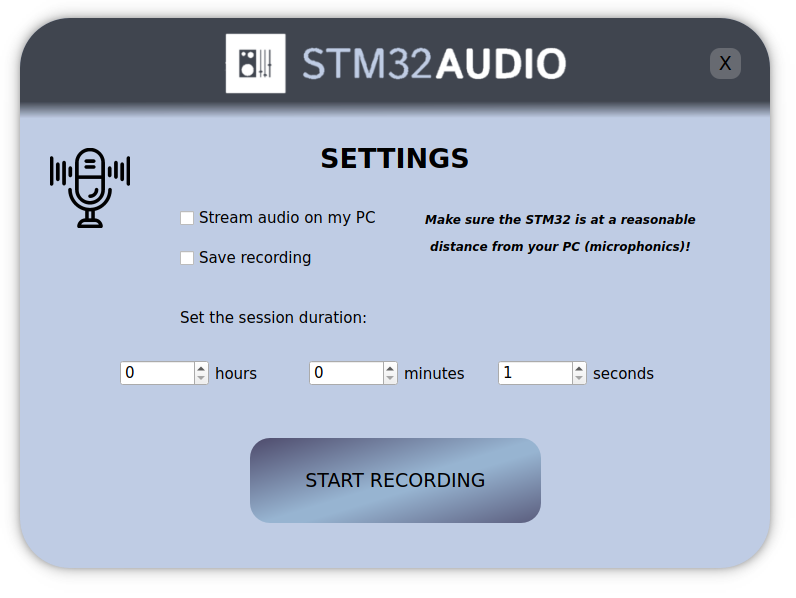
\includegraphics[width=\linewidth]{imgs/params_form}
	\caption{Sučelje za podešavanje parametara}
	\label{fig:params_form}
\end{figure}

Gumb \textit{Start} pokreće Bluetooth skeniranje uređaja na računalu. Ako nije pronađen uređaj s kojim se računalo može upariti, sustav obavještava korisnika te omogućuje ponovno skeniranje uređaja. 

Nakon uparivanja s pronađenim uređajem, pokreće se snimanje zvuka na mikrokontroleru. Korisničko sučelje ispisuje na ekranu prethodno postavljene parametre snimanja i preostalo vrijeme do kraja snimanja. Po završetku primljeni se zvučni zapis pohranjuje obliku \textit{RAW} datoteke, koja se zatim sprema u direktorij \textit{audioDumps}. Svaki zvučni zapis u svom nazivu sadrži vremensku oznaku početka snimanja. 

Snimanje je moguće pokrenuti ponovno pritiskom na gumb \textit{Start}, ali s ranije definiranim parametrima.

\vspace*{3\baselineskip}
 
%%
%mini slikice%
\begin{figure}[ht]
	\begin{minipage}[t]{0.4\textwidth}
		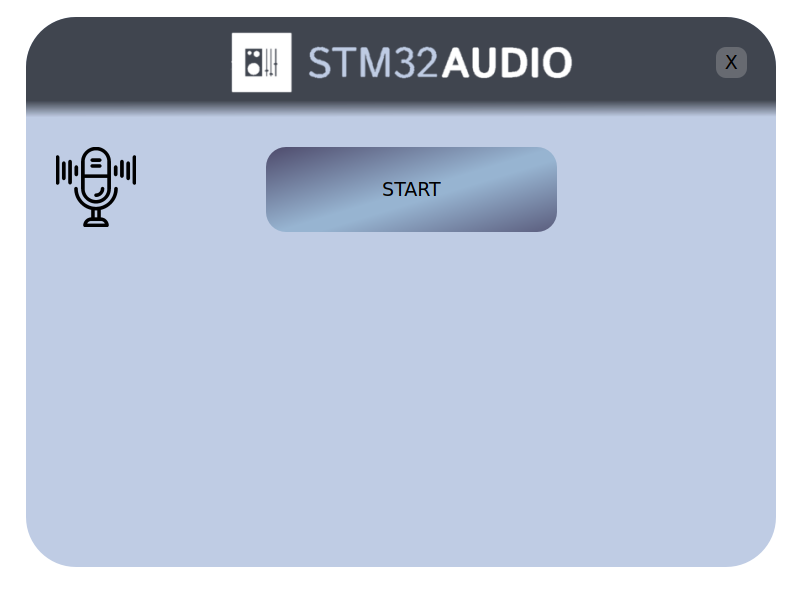
\includegraphics[width=\linewidth]{imgs/recording_form}
		\caption{Prije pokretanja snimanja}
		\label{fig:recording_form}
	\end{minipage}
	\hspace*{\fill}
	\begin{minipage}[t]{0.4\textwidth}
		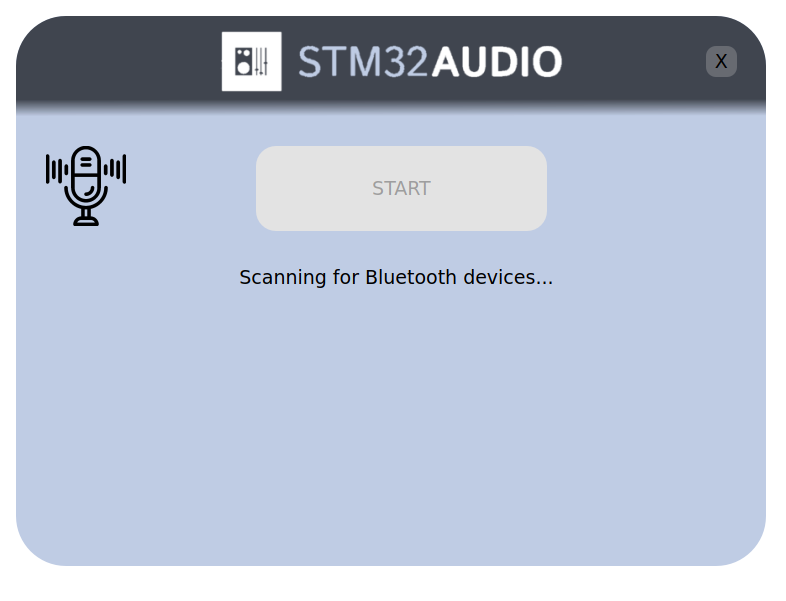
\includegraphics[width=\linewidth]{imgs/recording_form_2}
		\caption{Skeniranje uređaja}
		\label{fig:recording_form_2}
	\end{minipage}
\end{figure}

\begin{figure}[ht]
	\begin{minipage}[t]{0.4\textwidth}
	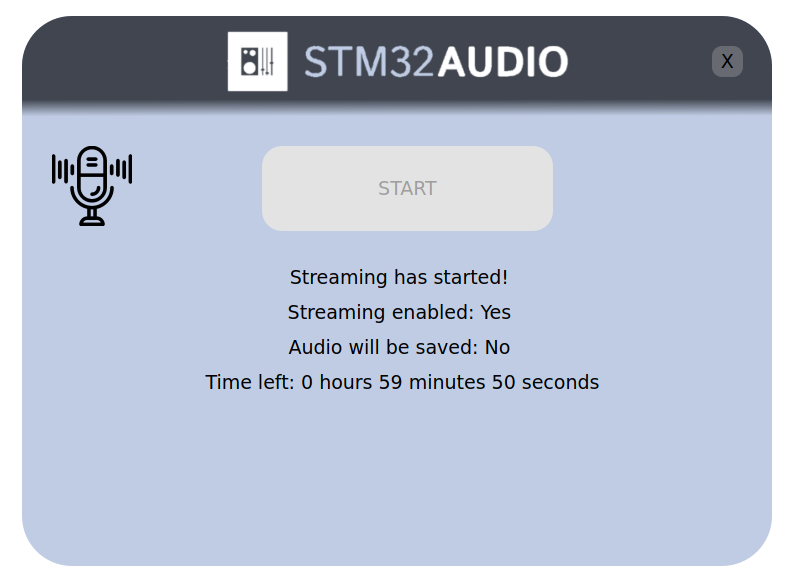
\includegraphics[width=\linewidth]{imgs/recording_form_3}
	\caption{Snimanje zvuka}
	\label{fig:recording_form_3}
	\end{minipage}
	\hspace*{\fill}
	\begin{minipage}[t]{0.4\textwidth}
		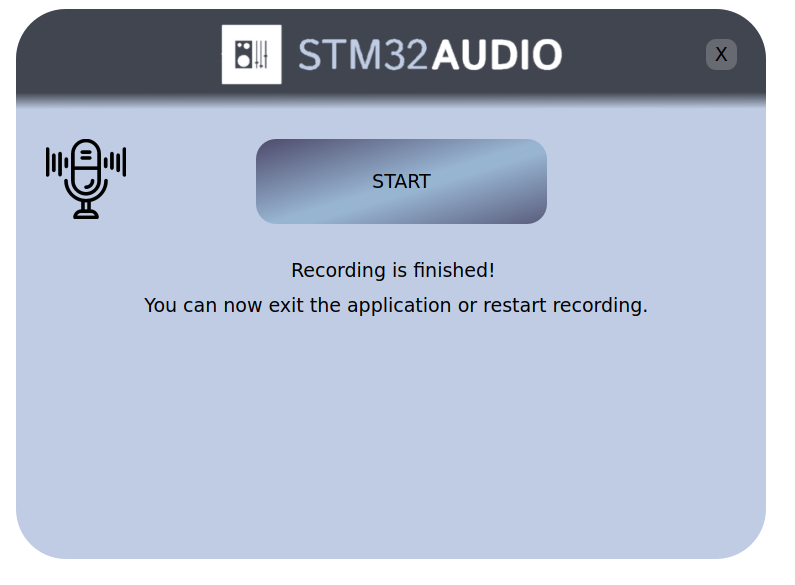
\includegraphics[width=\linewidth]{imgs/recording_form_4}
		\caption{Završetak snimanja}
		\label{fig:recording_form_4}
	\end{minipage}
\end{figure}
%end mini slikice%
%%


Glavni prozor i ostali elementi korisničkog sučelja konfiguriraju se u klasi \textit{Ui\_Form}, odnosno u njezinoj funkciji \lstinline|setupUi()|, koja kao parametar prima objekt \textit{Form}. Taj objekt nasljeđuje dvije klase - \textit{QWidget}, kao glavni prozor s grafičkim komponentama, i samu klasu \textit{Ui\_Form}, kako bi se glavni prozor mogao pomicati povlačenjem miša. 

\begin{lstlisting}[caption={Definicija klase \textit{Form} i njezin konstruktor}, language=Python]
	class Form(QtWidgets.QWidget, Ui_Form):
		def __init__(self, parent=None):
			super(Form, self).__init__(parent)
			self.setupUi(self)
			self.setMouseTracking(True)
\end{lstlisting}

Također, definiraju se dva objekta za praćenje vremena:
\begin{enumerate}
	\item \textit{QTimer}: pokreće se u trenutku početka snimanja zvuka i trajanje mu je određeno na prethodnom sučelju. Služi za prikaz preostalog vremena i signalima je povezan s metodom \lstinline|finished()| koja ispisuje poruku o završetku snimanja.
	\item \textit{QBasicTimer}: služi za osvježavanje grafičkog prikaza svake sekunde. Zaustavlja se istekom vremena postavljenog objektom \textit{QTimer}, odnosno aktiviranjem metode \lstinline|finished()|. Povezan je signalima s funkcijom \lstinline|timerEvent()| koja poziva metodu \lstinline|update_gui()| za ponovno iscrtavanje sučelja.
\end{enumerate}

Za pokretanje korisničkog sučelja potrebno je najprije napraviti instancu objekta \textit{QApplication} koja upravlja glavnim postavkama i tokom kontrole GUI aplikacije. \textit{QApplication} sadrži glavnu petlju događaja, gdje se obrađuju i šalju svi događaji iz prozorskog sustava i drugih izvora. Također upravlja inicijalizacijom, finalizacijom aplikacije i pruža upravljanje sesijom. Osim toga, \textit{QApplication} obrađuje većinu postavki za cijeli sustav i aplikaciju. Za bilo koju GUI aplikaciju koja koristi \textit{Qt}, postoji točno jedan objekt \textit{QApplication}, bez obzira na broj prozora. 

Metoda \lstinline|exec_()| pokreće glavnu petlju događaja i čeka dok se ne pozove \lstinline|exit| funkcija. Potrebno je pozvati ovu funkciju za početak rukovanja događajima. Glavna petlja događaja prima događaje iz prozorskog sustava i šalje ih widgetima aplikacije. Glavna petlja događaja prima događaje iz prozorskog sustava i šalje ih elementima  aplikacije.

\begin{lstlisting}[caption={Naredbe za pokretanje korisničkog sučelja}, language=Python]
	import sys
	app = QtWidgets.QApplication(sys.argv)
	w = Form()
	w.show()
	sys.exit(app.exec_())
\end{lstlisting}


\section{Višedretvenost sučelja i programske potpore}

PyQt aplikacije s grafičkim korisničkim sučeljem imaju glavnu dretvu koja pokreće glavnu petlju događaja i GUI. Pokrene li se dugotrajni zadatak u ovoj dretvi, GUI će se zamrznuti sve dok se zadatak ne izvrši. Za to vrijeme korisnik ne može komunicirati s aplikacijom, niti se prikaz sučelja može mijenjati tijekom izvođenja zadatka. Stoga je izvođenje dugotrajnih zadataka potrebno odvojiti od rada korisničkog sučelja.

U ovoj aplikaciji prikaz sučelja i programska potpora koja obavlja povezivanje Bluetoothom i snimanje zvuka izvršavaju se paralelno, stoga ih je potrebno izvoditi simultano u dvjema dretvama koje međusobno komuniciraju. Iako Python u svojoj biblioteci nudi module za rad s dretvama, u ovoj je aplikaciji korištena klasa \textit{QtThread} koja se nalazi u okviru PyQt radi povezivanja rada dretvi sa signalima i događajima.

PyQt aplikacije imaju dvije vrste dretvi:
\begin{itemize}
	\item Glavna dretva
	\item dretve \textit{Worker}
\end{itemize}

Glavna dretva aplikacije uvijek postoji te se još naziva i GUI dretva. S druge strane, dretve tipa \textit{worker} ovise o potrebama aplikacije i može ih biti proizvoljno mnogo. One su sekundarne dretve koje se mogu koristiti za rasterećivanje glavnog programa i odvajanje dugotrajnih zadataka iz glavne dretve, čime se sprječava smrzavanje korisničkog sučelja. 

Svaki objekt \textit{QThread} upravlja jednom dretvom unutar programa i njihov rad započinje metodom \lstinline|run|. Ta metoda pokreće petlju događaja unutar dretve pozivanjem funkcije \lstinline|exec|. Važno je naglasiti da objekt \textit{QThread} nije dretva sam po sebi, nego je omotač oko dretve operacijskog sustava. Prava dretva kreira se pozivom funkcije \lstinline|QThread.start()|.

Klasa \textit{Worker} nasljeđuje klasu \textit{QObject} i u nju je smještena programska potpora za povezivanje računala s mikrokontrolerom. Također su definirana tri signala koja komuniciraju s glavnom dretvom - jedan koji signalizira kraj izvođenja procesa, drugi za ažuriranje tekstualnog prikaza, i treći koji signalizira početak snimanja zvuka. Svaki od signala pozivom metode \lstinline|emit()| emitira signal glavnoj petlji o vlastitoj promjeni. 

\begin{lstlisting}[caption={Klasa \textit{Worker}}, language=Python]
	class Worker(QObject):
		# Class for running BLE 
		finished = pyqtSignal()
		textlabel = pyqtSignal(str)
		stream = pyqtSignal()
	
		def run(self):
			self.textlabel.emit("Scanning for devices...")
			# ... code for BLE connection ... 
			return
\end{lstlisting}

Isječak koda 4.4 prikazuje princip povezivanja glavne, GUI dretve s dretvom tipa \textit{worker} koja povezuje rad mikrokontrolera i računala.

Za početak je potrebno stvoriti instance klasa \textit{QThread} i \textit{Worker}. Nakon toga, funkcijom \lstinline|moveToThread()| funkcionalnost klase \textit{Worker} prebacuje se u objekt \textit{QThread} koji će se izvršavati neovisno o GUI dretvi. Zatim je potrebno povezati signale dretve s funkcijama koje će se izvršiti pri emisiji signala. Naposljetku, izvršavanje dretve započinje pokretanjem metode \lstinline|start()| nad objektom \textit{QThread}, što ujedno i emitira \lstinline|started| signal koji je povezan s metodom \lstinline|run()| objekta \textit{Worker}. Time je započet rad te klase u odvojenoj dretvi bez ikakve ovisnosti o glavnoj dretvi s korisničkim sučeljem.

\begin{lstlisting}[caption={Povezivanje glavne dretve s dretvom tipa \textit{worker}}, language=Python]
	# Step 1: Create a QThread object
	self.thread = QThread()
	# Step 2: Create a worker object
	self.worker = Worker()
	# Step 3: Move worker to the thread
	self.worker.moveToThread(self.thread)
	# Step 4: Connect signals and slots
	self.thread.started.connect(self.worker.run)
	self.worker.finished.connect(self.thread.quit)
	...
	# Step 5: Start the thread
	self.thread.start()
\end{lstlisting}


\eject
\chapter{Obrada audio signala}

Nakon otvaranja audio datoteke, vrši se obrada zvučnog signala. Audio biblioteka \textit{SoundFile} koristi se za učitavanje audio datoteke te, pozivom \lstinline|sf.read(file_path)| dobivaju se matrica amplituda i frekvencija uzorkovanja. Dobivena matrica reprezentacija je audio signala u vremenskoj domeni, odnosno prikazuje glasnoću (amplitudu) zvuka dok se mijenja u vremenu. Amplituda jednaka nuli označava tišinu.

Za analizu odnosa amplitude i frekvencije signala potrebno transformirati signal u frekvencijsku domenu kako bi se prikazalo koje frekvencije se nalaze u signalu. Fourierovom transformacijom signal se dekomponira u odgovarajuće frekvencije. \textit{Scipy} biblioteka sadrži ugrađenu funkciju za brzu Fourierovu transformaciju.

Dobivene matrice iscrtavaju se grafički pomoću biblioteke \textit{matplotlib}. Ograničen je prikaz frekvencija na 2000 Hz...


\begin{figure}[ht]
	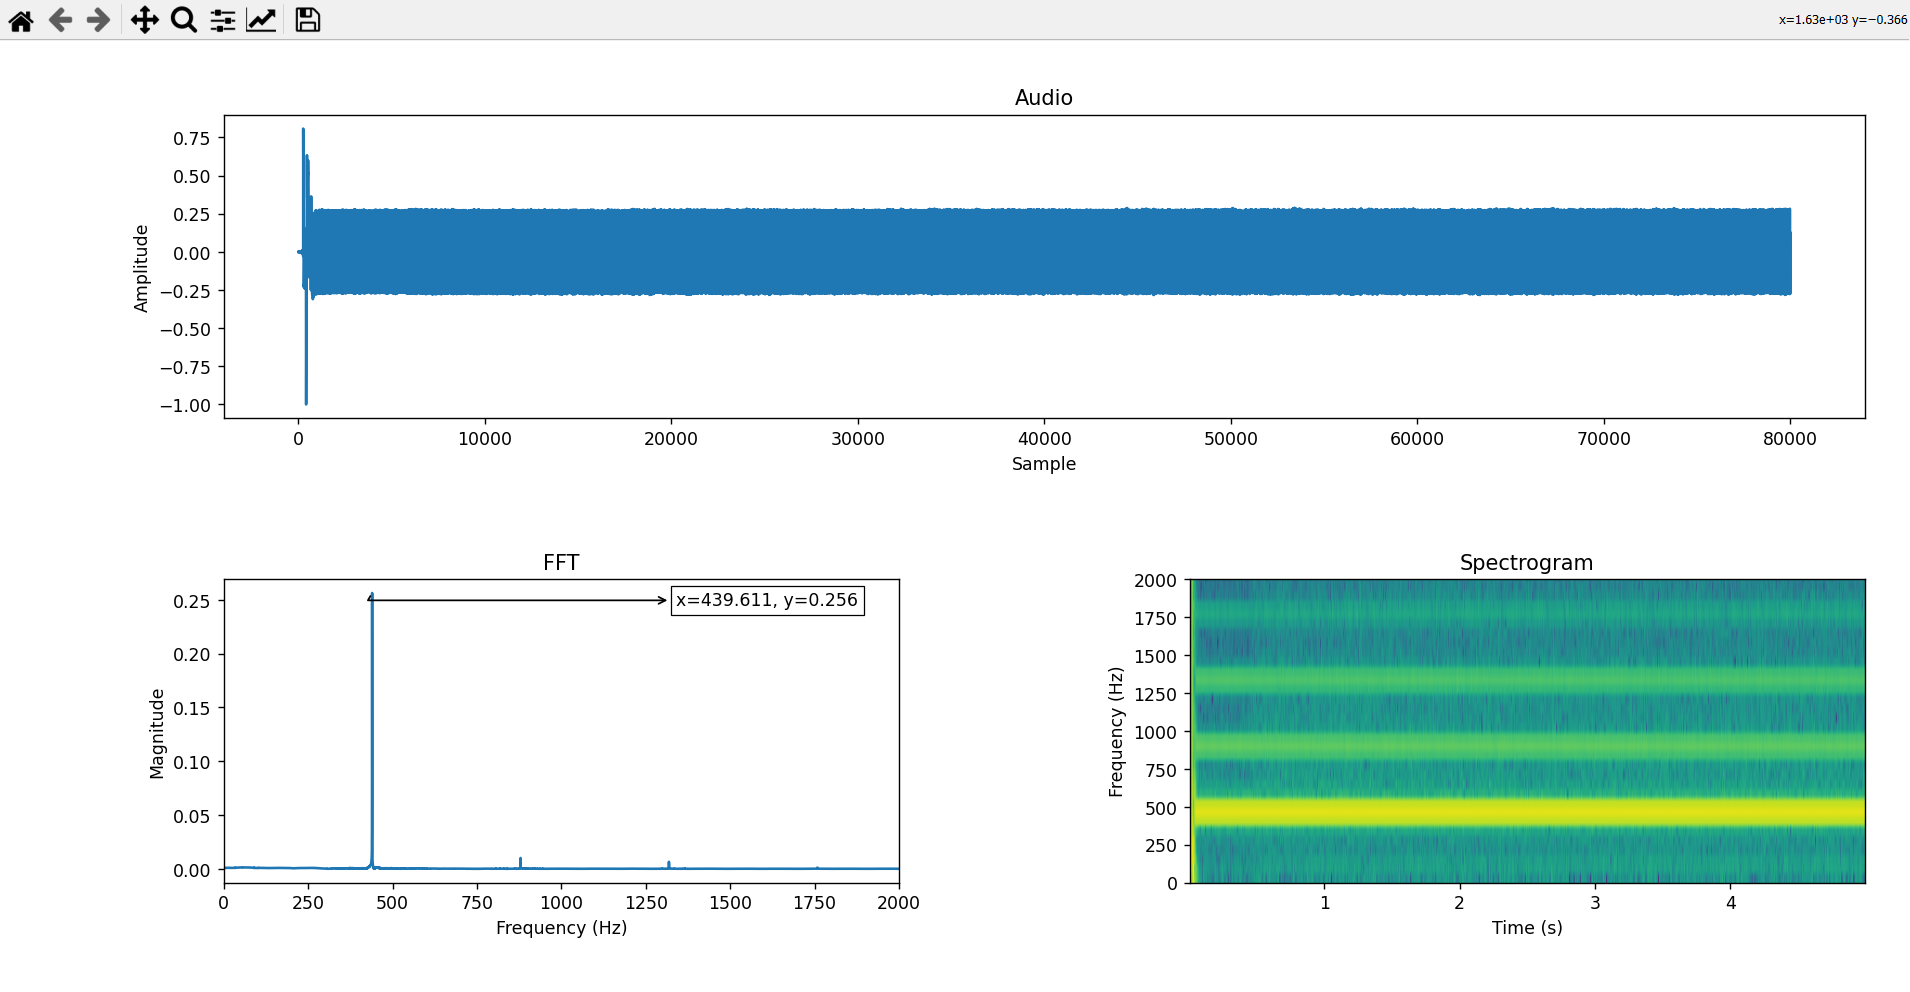
\includegraphics[width=\linewidth]{imgs/analyse_example}
	\caption{Primjer prikaza analize audiozapisa}
	\label{fig:analyse_example}
\end{figure}

\chapter{Zaključak}



\bibliography{literatura}{}
\bibliographystyle{fer}

\begin{sazetak}
U ovom radu implementiran je sustav za prijam, prikaz i obradu audio signala korištenjem razvojnog sustava STM32WB5MM-DK. Korištene su biblioteke koje omogućavaju snimanje zvuka MEMS mikrofonom na razvojnom sustavu. Korišteno je BLE sučelje za prijenos audio signala s razvojnog sustava na računalo. Razvijeno je grafičko korisničko sučelje za snimanje zvuka i vizualizaciju ranije snimljenih podataka korištenjem razvojnog alata \textit{PyQt}. Aplikacija se izvodi na operacijskom sustavu Linux. Provedena je analiza zvučnih zapisa hrkanja snimljenih razvijenim sustavom. 

\kljucnerijeci{STM32WB5MM-DK, BLE, MEMS mikrofon, korisničko sučelje, obrada audio signala, hrkanje}
\end{sazetak}

% TODO: Navedite naslov na engleskom jeziku.
\engtitle{Audio Signal Transmission Using BLE Interface of STM32WB5MM-DK Development Kit}
\begin{abstract}
This thesis describes an implementation of a system for receiving, displaying and analysis of audio signal using STM32WB5MM-DK development board. Libraries that enable audio recording with a MEMS microphone on the development board have been used. BLE interface is used for signal transfer from the STM32WB5MM-DK to the computer. A graphical user interface has been developed for audio recording and audio signal visualization, using \textit{PyQt} development tools. The application runs on the Linux operating system. Analysis of snoring audio recorded with the developed system has been performed. 

\keywords{STM32WB5MM-DK, BLE, MEMS microphone, user interface, audio signal processing, snoring}
\end{abstract}

\end{document}
